%%%%%%%%%%%%%%%%%%%%%%%%%%%%%%%%%%%%%%%%%%%%%%%%%%%%%%%%%%%%%%%%%%%%%%%%%%%%% %
% crowdsourcing.tex
%
% Ian Roberts, February 2014
%
% $Id: uima.tex,v 1.3 2006/10/21 11:44:47 ian Exp $
%
%%%%%%%%%%%%%%%%%%%%%%%%%%%%%%%%%%%%%%%%%%%%%%%%%%%%%%%%%%%%%%%%%%%%%%%%%%%%%


%%%%%%%%%%%%%%%%%%%%%%%%%%%%%%%%%%%%%%%%%%%%%%%%%%%%%%%%%%%%%%%%%%%%%%%%%%%%%
\chapt[chap:crowd]{Crowdsourcing Data with GATE}
\markboth{Crowdsourcing Data with GATE}{Crowd-Sourcing Data with GATE}
%%%%%%%%%%%%%%%%%%%%%%%%%%%%%%%%%%%%%%%%%%%%%%%%%%%%%%%%%%%%%%%%%%%%%%%%%%%%%
\nnormalsize

To develop high-performance language processing applications, you need training
data. Traditionally that means recruiting a small team of experts in your
chosen domain, then several iterations developing annotation guidelines,
training your annotators, doing a test run, examining the results, refining the
guidelines until you reach an acceptable level of inter-annotator agreement,
letting the annotators loose on the full corpus, cross-checking their
results\ldots  Clearly this can be a time-consuming and expensive process.

An alternative approach for some annotation tasks is to \emph{crowdsource} some
or all of your training data. If the task can be defined tightly enough and
broken down into sufficiently small self-contained chunks, then you can take
advantage of services such as Amazon Mechanical
Turk\footnote{\htlinkplain{https://www.mturk.com/}} to farm out the tasks to a
much larger pool of users over the Internet, paying each user a small fee per
completed task.  For the right kinds of annotation tasks crowdsourcing can be
much more cost-effective than the traditional approach, as well as giving a
much faster turn-around time (since the job is shared among many more people
working in parallel).

This \chapthing{} describes the tools that GATE Developer provides to assist in
crowdsourcing data for training and evaluation.  GATE provides tools for two
main types of crowdsourcing task:

\begin{itemize}
\item \emph{annotation} -- present the user with a snippet of text (e.g.
  a sentence) and ask them to mark all the mentions of a particular annotation
  type.
\item \emph{classification} -- present the user with a snippet of text
  containing an existing annotation with several possible labels, and ask them
  to select the most appropriate label (or ``none of the above'').
\end{itemize}

%%%%%%%%%%%%%%%%%%%%%%%%%%%%%%%%%%%%%%%%%%%%%%%%%%%%%%%%%%%%%%%%%%%%%%%%%%%%%
\sect[sec:crowd:basics]{The Basics}

The GATE crowdsourcing tools are based on the \emph{Figure Eight}
platform\footnote{\htlinkplain{http://figure-eight.com}} (formerly
known as CrowdFlower).  To get the most out of the GATE tools it is
first necessary to understand a few pieces of Figure Eight terminology.

\begin{itemize}
\item a \emph{job} is the container which represents a single end-to-end
  crowdsourcing process.  It defines the input form you want to present to your
  workers, and holds a number of units of work.
\item a \emph{unit} is a single item of work, i.e. a single snippet (for
  annotation jobs) or a single entity (for classification jobs).  Figure Eight
  presents several units at a time to the user as a single \emph{task}, and
  users are paid for each task they successfully complete.
\item a \emph{gold} unit is one where the correct answer is already known in
  advance.  Gold units are the basis for determining whether a task has been
  completed ``successfully'' -- when a job includes gold units, Figure Eight
  includes one gold unit in each task but does not tell the user which one it
  is, and if they get the gold unit wrong then the whole task is disregarded.
  You can track users' performance through the Figure Eight platform and ignore
  results from users who get too many gold units wrong.
\end{itemize}

Figure Eight provides a web interface to build jobs in a browser, and also a
REST API for programmatic access.  The GATE tools use the REST API, so you will
need to sign up for a Figure Eight account and generate an API key which you
will use to configure the various processing resources.

To access the GATE crowdsourcing tools, you must first load the
\verb!Crowd_Sourcing! plugin.  This plugin provides four PR types, a ``job
builder'', ``results importer'' and ``consensus builder'' for each of the two
supported styles of crowdsourcing job.

%%%%%%%%%%%%%%%%%%%%%%%%%%%%%%%%%%%%%%%%%%%%%%%%%%%%%%%%%%%%%%%%%%%%%%%%%%%%%
\sect[sec:crowd:classification]{Entity classification}

The ``entity classification'' job builder and results importer PRs are intended
for situations where you have pre-annotated entities but each entity could have
one of several different labels.  Examples could be:

\begin{itemize}
\item a term recognintion system that has established which spans of text are
  candidate terms but not what class of term each annotation represents.
\item annotation with respect to an ontology, when the same string could match
  one of several different ontology concepts.
\end{itemize}

In the first case, the set of available labels would be constant, with the same
set of options presented for every unit.  In the second case each annotation
would supply its own set of options (there may also be ``common options''
available for every annotation, such as ``none of the above'').

\subsect[sec:crowd:classification:create]{Creating a classification job}

To start a new classification job, first load the \verb!Crowd_Sourcing! plugin,
then create a new instance of the ``Entity Classification Job Builder'' PR.
The PR requires your Figure Eight API key as an init-time parameter.

Right-clicking on the newly-created PR in the resources tree will offer the
option to ``Create a new Figure Eight job'', which presents a dialog to
configure the settings of the new job (see
figure~\ref{fig:crowd:new-classification-job}).  The available options are as
follows:

\begin{figure}[tb]
  \centering
  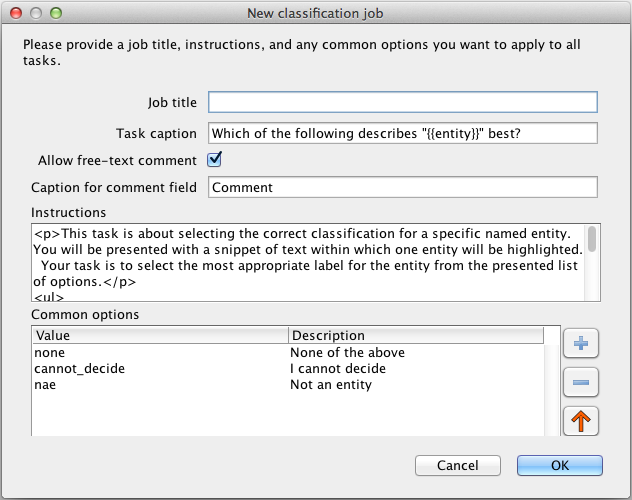
\includegraphics[width=0.5\textwidth]{new-classification-job-dialog.png}
  \caption{Setting options to create a new classification job}
  \label{fig:crowd:new-classification-job}
\end{figure}

\begin{description}
\item[Job title] a descriptive title for this job %TODO check does this appear to the workers?
\item[Task caption] the ``question'' that the user will be asked.  This is
  shown above the snippet showing the entity in context, and may include the
  placeholder \verb!{{entity}}! (including the double braces) which will be
  replaced by the text covered by the target entity annotation.
\item[Allow free-text comment] whether to offer a free-text field to the
  annotator in addition to the selectable options.  This could be used for a
  variety of purposes, for example for the annotator to suggest an alternative
  if none of the options offered are correct, to state how confident they are
  about their response, or to higlight perceived errors in the data.
\item[Caption for comment field] the caption to be displayed for the free-text
  field.  The appropriate caption depends on the purpose of the field, for
  example if the last of the ``common options'' (see below) is ``Other'' then
  the comment field caption could be ``please specify''.
\item[Instructions] detailed instructions that will be shown to workers.  In
  contrast to the caption, which is shown as part of each unit, the
  instructions appear just once on each task page, and are in a collapsible
  panel so the user can hide them once they are confident that they understand
  the task.  The instructions are rendered as HTML, which allows them to
  include markup but also means that characters such as \verb!&! and \verb!<!
  must be escaped as HTML entity references.
\item[Common options] options that will be available for \emph{all} units, in
  addition to unit-specific options taken from the target annotation.  These
  common options appear below the unit-specific options (if any) and are
  presented in the order specified here.  Use the \verb!+! and \verb|-| buttons
  to add and remove options, and the arrows to change the order.  For each row
  in the table, the ``Value'' column is the value that will be submitted as the
  answer if the user selects this option, the ``Description'' is the string
  that will be shown to the user.  It is a good idea to include details in the
  instructions to explain the common options.
\end{description}

Clicking ``OK'' will make calls to the Figure Eight REST API to create a job
with the given settings, and store the resulting job ID so the PR can be used
to load units into the job.

\subsect[sec:crowd:classification:data]{Loading data into a job}

When added to a corpus pipeline application, the PR will read annotations from
documents and use them to create units of work in the Figure Eight job.  It is
highly recommended that you store your documents in a persistent corpus in a
serial datastore, as the PR will add additional features to the source
annotations which can be used at a later date to import the results of the
crowdsourcing job and turn them back into GATE annotations.

The job builder PR has a few runtime parameters:
\begin{description}
\item[contextASName/contextAnnotationType] the annotation set and type
  representing the snippets of text that will be shown as the ``context''
  around an entity.  Typically the ``context'' annotation will be something
  like ``Sentence'', or possibly ``Tweet'' if you are working with Twitter
  data.
\item[entityASName/entityAnnotationType] the annotation set and type
  representing the individual entities to be classified.  Every ``entity''
  annotation must fall within the span of at least one ``context'' annotation --
  entities that are not covered by \emph{any} context annotation will be
  ignored (and a warning logged for debugging purposes), and if there is more
  than one context annotation that covers an entity (e.g. HTML \verb!div! tags
  that are nested) then the shortest annotation from among the alternatives
  will be the one chosen.
\item[jobId] the unique identifier of the Figure Eight job that is to be
  populated.  This parameter is filled in automatically when you create a job
  with the dialog described above.
\item[skipExisting] if true (the default), entity annotations that already have
  a \verb!cf_unit! feature (indicating that they have already been processed by a
  previous run of this PR) will be ignored.  This means that if the loading
  process fails part way through it can simply be re-run over the same corpus
  and it will continue from where it left off without creating duplicate units.
\end{description}

The number and format of the options presented to the user, and the marking of
annotations as ``gold'' is handled by a number of conventions governing the
features that each entity annotation is expected to have.  Getting the
annotations into the required format is beyond the scope of the
\verb!Crowd_Sourcing! plugin itself, and will probably involve the use of
custom JAPE grammars and/or Groovy scripts.

The job builder expects the following features on each entity annotation:
\begin{description}
\item[options] the classification options that are specific to this unit.  If
  this feature is supplied its value must take one of two forms, either:
  \begin{enumerate}
  \item a \verb!java.util.Collection! of values (typically strings, but any
    object with a sensible \verb!toString()! representation can be used).
  \item a \verb!java.util.Map! where a \emph{key} in the map is the value to be
    submitted by the form if this option is selected, and the corresponding
    \emph{value} is the description of the option that will be displayed to the
    user.  For example, if the task is to select an appropriate URI from an
    ontology then the key would be the ontology URI and the value could be an
    \verb!rdfs:label! for that ontology resource in a suitable language.
  \end{enumerate}
  If this feature is omitted, then only the ``common options'' configured for
  the job will be shown.
\item[default] the option that should be selected by default when this unit is
  shown to a worker.  The value must match one of the ``options'' for this
  unit (a \emph{key} if the options are a map) or one of the ``common options''
  for the job.  If omitted, no value will be selected by default.
\item[detail] any additional details to be shown to the worker along with the
  snippet text and highlighted entity.  This value is interpreted as HTML, and
  could be used for many purposes.  As one example, there is a JAPE grammar in
  \texttt{plugins/Crowd\_Sourcing/resources} to create an HTML list of links
  from the content of any \verb!Url! annotations contained within the snippet.
\item[correct] the ``correct answer'' if this annotation represents a gold
  unit, which must match one of the ``options'' for this unit (a \emph{key} if
  the options are given as a map) or one of the job's configured ``common
  options''.  If omitted the unit is not marked as gold.
\item[reason] for gold units, the reason \emph{why} the correct answer is
  correct.  This will be displayed to users who select the wrong answer for
  this unit to provide feedback.
\item[entity/leftContext/rightContext] Snippet text to be used. If any of 
  these values are omitted, the text will instead be taken from the document
  content for the annotations indicated by contextAnnotationType and 
  entityAnnotationType annotation.

\end{description}

Note that the options will be presented to the workers in the order they are
returned by the collection (or the map's \verb!entrySet()!) iterator.
If this matters then you should consider using a collection or map type with
predictable iteration order (e.g. a \verb!List! or \verb!LinkedHashMap!).  In
particular it is often a good idea to randomize the ordering of options -- if
you always put the most probable option first then users will learn this and
may try to ``beat the system'' by always selecting option 1 for every unit.

The ID of the created unit will be stored as an additional feature named
\verb!cf_unit! on the entity annotation.

\subsect[sec:crowd:classification:import]{Importing the results}

Once you have populated your job and gathered judgments from human workers, you
can use the ``Entity Classification Results Importer'' PR to turn those
judgments back into GATE annotations in your original documents.

As with the job builder, the results importer PR has just one initialization
parameter, which is your Figure Eight API key, and the following runtime
parameters:
\begin{description}
\item[entityASName/entityAnnotationType] the annotation set and type
  representing the entities that have been classified.  Each entity annotation
  should have a \verb!cf_unit! feature created by the job builder PR.
\item[resultASName/resultAnnotationType] the annotation set and type where
  annotations corresponding to the judgments of your annotators should be
  created.
\item[answerFeatureName] (default ``answer'') the name of the feature on each
  result annotation that will represent the answer selected by the annotator.
\item[jobId] the ID of the Figure Eight job whose results are being imported
  (copy the value from the corresponding job builder PR).
\end{description}

When run, the results importer PR will call the Figure Eight REST API to
retrieve the list of judgments for each unit in turn, and then create one
annotation of the target type in the target annotation set (as configured by
the ``result'' runtime parameters) for each judgment -- so if your job required
three annotators to judge each unit then the unit will generate three output
annotations, all with the same span (as each other and as the original input
entity annotation).  Each generated annotation will have the following
features:
\begin{description}
\item[cf\_judgment] the ``judgment ID'' -- the unique identifier assigned to
  this judgment by Figure Eight.
\item[worker\_id] the Figure Eight identifier for the worker who provided this
  judgment.  There is no way to track this back directly to a specific human
  being, but it is guaranteed that two judgments with the same worker ID were
  performed by the same person.
\item[trust] the worker's ``trust score'' assigned by Figure Eight based on the
  proportion of this job's gold units they answered correctly.  The higher the
  score, the more reliable this worker's judgments.
\item[comment] the contents of the free-text comment field supplied by the
  user, if this field was enabled when the job was created.  If the user leaves
  the comment field empty this feature will be omitted.
\end{description}

In addition, the feature named by the \verb!answerFeatureName! parameter (by
default ``answer'') will hold the answer selected by the user -- this will be
one of the option values (a map key if the options were provided as a map) or
one of the common options configured when the job was created.

Since each generated annotation tracks the judgment ID it was created from,
this PR is idempotent -- if you run it again over the same corpus then new
annotations will be created for new judgments only, you will not get duplicate
annotations for judgments that have already been processed.


\subsect[sec:crowd:classification:adjudication]{Automatic adjudication}

Once you have imported the human judgments from Figure Eight back into GATE
annotations, a common next step is to take the multiply-annotated entities and
attempt to build a single ``consensus'' set of the classifications where enough
of the annotators agree.  The simplest form of automatic adjudication is the
majority-vote method, where classifications are automatically accepted if at
least $n$ out of $m$ annotators agree on them.  Entities that do not have the
required level of agreement cannot be accepted automatically and must be double
checked somehow, either directly within GATE Developer or via a second round of
crowdsourcing.

This approach is implemented by the ``Majority-vote consensus builder
(classification)'' PR.  It takes the following runtime parameters:
\begin{description}
\item[originalEntityASName/entityAnnotationType] the annotation set and type
  representing the original entities that were used to generate the units sent
  for annotation by the crowd.
\item[resultASName/resultAnnotationType] the annotation set and type where
  annotations corresponding to the judgments of your annotators were created by
  the results importer.
\item[answerFeatureName] (default ``answer'') the name of the feature on each
  result annotation that represents the answer selected by the annotator.
\item[minimumAgreement] the minimum number of annotators who must agree on the
  same option in order for it to be eligible for the consensus set.  Usually
  this threshold would be set at more than half the total number of judgments
  for each entity, so at most one option can meet the threshold, but this is
  not required.  In any case, an entity is only ever eligible for the consensus
  set if \emph{exactly one} option meets the threshold.
\item[consensusASName] (default ``crowdConsensus'') the annotation set where
  consensus annotations should be created, for the entities that meet the
  agreement threshold.
\item[disputeASName] (default ``crowdDispute'') the annotation set where
  disputed annotations should be placed, for the entities that do not meet the
  agreement threshold (if the threshold is less than half the total number of
  annotators it is possible for more than one option to meet the threshold --
  these cases will also be considered disputed).
\item[noAgreementAction] what to do with disputed entities.  This is discussed
  in more detail below.
\end{description}

When run over a corpus, the PR will look at each of the original entity
annotations in turn and count up the number of annotators who selected each of
the available options (including common options specified at the job level).
If there is \emph{exactly} one option on which at least \emph{minimumAgreement}
annotators agree, then it will create a single annotation in the consensus
annotation set, whose type is \emph{resultAnnotationType} and whose
\emph{answerFeatureName} feature is the selected option.

If there is no agreement (either no option meets the threshold, or more than
one option in the case when the threshold is below 50\%), then the PRs action
is determined by the \emph{noAgreementAction} parameter:
\begin{description}
\item[resolveLocally] all the judgment annotations are copied from the result
  set into the dispute set, so they can be inspected locally in GATE Developer
  (typically using the annotation stack view).
\item[reAnnotateByCrowd] the \emph{original} entity annotation is copied to the
  dispute set, with two modifications:
  \begin{itemize}
  \item its \verb!cf_unit! feature is removed
  \item its \verb!options! feature is restricted to the subset of the original
    options that were selected by at least one of the annotators in the first
    round of annotation.
  \end{itemize}
\end{description}

In the \emph{reAnnotateByCrowd} case, the resulting entity annotations are
suitable to be imported into Figure Eight again for another round of
crowdsourced annotation, but this time highly ambiguous entities have a smaller
set of choices that will be presented to the workers.

%%%%%%%%%%%%%%%%%%%%%%%%%%%%%%%%%%%%%%%%%%%%%%%%%%%%%%%%%%%%%%%%%%%%%%%%%%%%%
\sect[sec:crowd:annotation]{Entity annotation}

The ``entity annotation'' job builder and results importer PRs are intended
for situations where you want people to mark occurrences of named entities in
plain text.  A number of simplifying assumptions are made to make this task
suitable for crowdsourcing:
\begin{itemize}
\item Text is presented in short snippets (e.g. one sentence or Tweet at a
  time).
\item Each job focuses on one specific entity type (if you want to annotate
  different entities you can do this by running a number of different jobs over
  the same corpus).
\item Entity annotations are constrained to whole tokens only, and there are no
  adjacent annotations (i.e. a contiguous sequence of marked tokens represents
  \emph{one} target annotation, and different annotations must be separated
  by at least one intervening token).  This is a reasonable assumption to make
  given the previous point, as adjacent entities of the same type will usually
  be separated by something (a comma, the word ``and'', etc.).
\end{itemize}

\subsect[sec:crowd:annotation:create]{Creating an annotation job}

To start a new annotation job, first load the \verb!Crowd_Sourcing! plugin,
then create a new instance of the ``Entity Annotation Job Builder'' PR.
The PR requires your Figure Eight API key as an init-time parameter.

Right-clicking on the newly-created PR in the resources tree will offer the
option to ``Create a new Figure Eight job'', which presents a dialog to
configure the settings of the new job (see
figure~\ref{fig:crowd:new-annotation-job}).  The available options are as
follows:

\begin{figure}[tb]
  \centering
  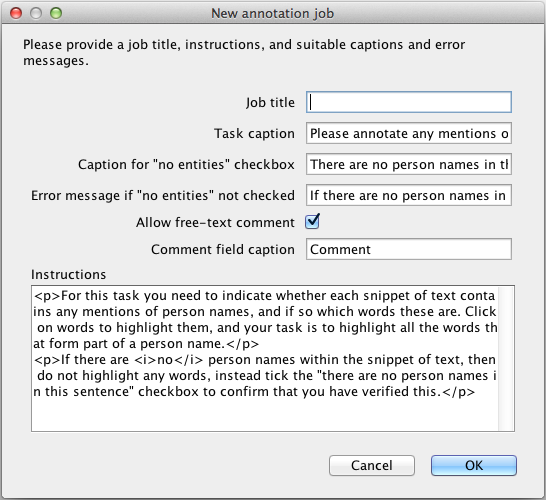
\includegraphics[width=0.5\textwidth]{new-annotation-job-dialog.png}
  \caption{Setting options to create a new annotation job}
  \label{fig:crowd:new-annotation-job}
\end{figure}

\begin{description}
\item[Job title] a descriptive title for this job %TODO check does this appear to the workers?
\item[Task caption] the ``question'' that the user will be asked, which should
  include the kind of annotations they are being asked to find.
\item[Caption for ``no entities'' checkbox] if the user does not select any
  tokens to annotate, they must explicitly click a checkbox to confirm that
  they believe there are no mentions in this unit.  This is done to distinguish
  between units that have not been attempted and units which have been
  attempted but for which the correct answer is ``nothing''.  This parameter is
  the caption shown for this checkbox, and should include the kind of
  annotations the user is being asked to find.
\item[Error message if ``no entities'' not checked] if the user attempts to
  submit a unit where they have not selected any tokens to annotate but have
  also not clicked the checkbox, this is the error message that will be shown.
  It should include the kind of annotations the user is being asked to find.
\item[Allow free-text comment] whether to offer a free-text field to the
  annotator in addition to the selectable options.  This could be used for a
  variety of purposes, for example for the annotator to state how confident
  they are about their response, or to higlight perceived errors in the data.
\item[Caption for comment field] the caption to be displayed for the free-text
  field.  The appropriate caption depends on the purpose of the field.
\item[Instructions] detailed instructions that will be shown to workers.  In
  contrast to the caption, which is shown as part of each unit, the
  instructions appear just once on each task page, and are in a collapsible
  panel so the user can hide them once they are confident that they understand
  the task.  The instructions are rendered as HTML, which allows them to
  include markup but also means that characters such as \verb!&! and \verb!<!
  must be escaped as HTML entity references.
\end{description}

The defaults assume a job to annotate person names within the context of a
single sentence, where the selection is done at the level of words (i.e. Token
annotations).  Figure~\ref{fig:crowd:sample-annotation-job} shows how the units
are presented to users.
\begin{figure}[tb]
  \centering
  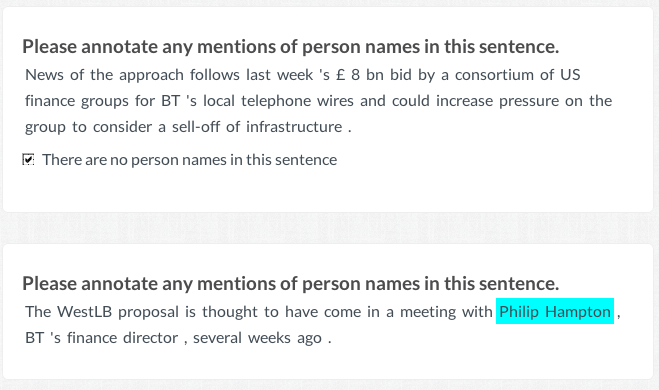
\includegraphics[width=0.5\textwidth]{example-cf-annotation-job.png}
  \caption{Example of how an annotation job is presented to workers}
  \label{fig:crowd:sample-annotation-job}
\end{figure}


Clicking ``OK'' will make calls to the Figure Eight REST API to create a job
with the given settings, and store the resulting job ID so the PR can be used
to load units into the job.

\subsect[sec:crowd:annotation:data]{Loading data into a job}

When added to a corpus pipeline application, the PR will read annotations from
documents and use them to create units of work in the Figure Eight job.  It is
highly recommended that you store your documents in a persistent corpus in a
serial datastore, as the PR will add additional features to the source
annotations which can be used at a later date to import the results of the
crowdsourcing job and turn them back into GATE annotations.

The job builder PR has a few runtime parameters:
\begin{description}
\item[snippetASName/snippetAnnotationType] the annotation set and type
  representing the snippets of text that will be shown to the user.  Each
  snippet is one unit of work, and typical examples would be ``Sentence'' or
  ``Tweet''.
\item[tokenASName/tokenAnnotationType] the annotation set and type representing
  ``tokens'', i.e. the atomic units that users will be asked to select when
  marking annotations.  The token annotations should completely cover all the
  non-whitespace characters within every snippet, and when presented to the
  user the tokens will be rendered with a single space between each pair.  In
  the vast majority of cases, the default value of ``Token'' will be
  the appropriate one to use.
\item[detailFeatureName] feature on the snippet annotations that contains any
  additional details to be shown to the worker along with the snippet tokens.
  This value is interpreted as HTML, and could be used for many purposes.  As
  one example, there is a JAPE grammar in
  \texttt{plugins/Crowd\_Sourcing/resources} to create an HTML list of links
  from the content of any \verb!Url! annotations contained within the snippet.
\item[entityASName/entityAnnotationType] the annotation set and type
  representing the annotations that the user is being asked to create.  Any
  already-existing annotations of this type can be treated as gold-standard
  data.
\item[goldFeatureName/goldFeatureValue] a feature name/value pair that is used
  to mark snippets that should become gold units in the job.  Any snippet
  annotation that has the matching feature is considered gold, and its
  contained entity annotations are used to construct the correct answer.  Note
  that it is possible for the correct answer to be that the snippet contains
  \emph{no} annotations, which is why we need an explicit trigger for gold
  snippets rather than simply marking as gold any snippet that contains at
  least one pre-annotated entity.  The default trigger feature is
  \verb!gold=yes!.
\item[goldReasonFeatureName] for gold units, this is the feature on the snippet
  annotation that contains the reason \emph{why} this particular unit has been
  annotated the way it has.  If the snippet contains annotations this should
  describe them and explain why they have been marked, if the snippet does
  \emph{not} contain annotations the reason should explain why (e.g. ``this
  text is a list of navigation links'').  Any user who gets this gold unit
  wrong will see the reason as feedback.
\item[jobId] the unique identifier of the Figure Eight job that is to be
  populated.  This parameter is filled in automatically when you create a job
  with the dialog described above.
\item[skipExisting] if true (the default), snippet annotations that already have
  an appropriate \verb!<Type>_unit_id! feature (indicating that they have
  already been processed by a previous run of this PR) will be ignored.  This
  means that if the loading process fails part way through it can simply be
  re-run over the same corpus and it will continue from where it left off
  without creating duplicate units.
\end{description}

When executed, the PR will create one unit from each snippet annotation in the
corpus and store the ID of the newly created unit on the annotation as a
feature named for the \verb!entityAnnotationType! with \verb!_unit_id! appended
to the end (e.g. \verb!Person_unit_id!).  This allows you to build several
different jobs from the same set of documents for different types of
annotation.

\subsect[sec:crowd:annotation:import]{Importing the results}

Once you have populated your job and gathered judgments from human workers, you
can use the ``Entity Annotation Results Importer'' PR to turn those
judgments back into GATE annotations in your original documents.

As with the job builder, the results importer PR has just one initialization
parameter, which is your Figure Eight API key, and the following runtime
parameters:
\begin{description}
\item[jobId] the ID of the Figure Eight job whose results are being imported
  (copy the value from the corresponding job builder PR).
\item[resultASName/resultAnnotationType] the annotation set and type where
  annotations corresponding to the judgments of your annotators should be
  created.  This annotation type \emph{must} be the same as the
  \verb!entityAnnotationType! you specified when creating the job, since the
  ``\texttt{\emph{resultAnnotationType}\_unit\_id}'' feature provides the link
  between the snippet and its corresponding Figure Eight unit.
\item[snippetASName/snippetAnnotationType] the annotation set and type
  containing the snippets whose results are to be imported.  Each snippet
  annotation must have an appropriate unit ID feature.
\item[tokenASName/tokenAnnotationType] the annotation set and type representing
  tokens.  The encoding of results from Figure Eight is based on the order of
  the tokens within each snippet, so it is imperative that the tokens used to
  import the results are the same as those used to create the units in the
  first place (or at least, that there are the same \emph{number} of tokens
  in the same order within each snippet as there were when the unit was
  created).
\item[annotateSpans] (boolean, default true) should adjacent tokens be merged
  into a single spanning annotation?
\end{description}

When run, the results importer PR will call the Figure Eight REST API to
retrieve the list of judgments for each unit in turn, and then create
annotations of the target type in the target annotation set (as configured by
the ``result'' runtime parameters) for each judgment, matching the tokens that
the annotator selected.  By default, a run of adjacent tokens will be treated
as a single annotation spanning from the start of the first to the end of the
last token in the sequence, but this can be disabled by setting
\emph{annotateSpans} to \verb!false!, in which case each token will be
annotated independently.  Each generated annotation will have the following
features:
\begin{description}
\item[cf\_judgment] the ``judgment ID'' -- the unique identifier assigned to
  this judgment by Figure Eight.
\item[worker\_id] the Figure Eight identifier for the worker who provided this
  judgment.  There is no way to track this back directly to a specific human
  being, but it is guaranteed that two judgments with the same worker ID were
  performed by the same person.
\item[trust] the worker's ``trust score'' assigned by Figure Eight based on the
  proportion of this job's gold units they answered correctly.  The higher the
  score, the more reliable this worker's judgments.
\item[comment] the contents of the free-text comment field supplied by the
  user, if this field was enabled when the job was created.  If the user leaves
  the comment field empty this feature will be omitted.
\end{description}

Since each generated annotation tracks the judgment ID it was created from,
this PR is idempotent -- if you run it again over the same corpus then new
annotations will be created for new judgments only, you will not get duplicate
annotations for judgments that have already been processed.

\subsect[sec:crowd:annotation:adjudication]{Automatic adjudication}

Once you have imported the human judgments from Figure Eight back into GATE
annotations, a common next step is to take the multiply-annotated entities and
attempt to build a single ``consensus'' set of the annotations where enough
of the annotators agree.  The simplest form of automatic adjudication is the
majority-vote method, where annotations are automatically accepted if at
least $n$ out of $m$ annotators agree on them.  Entities that do not have the
required level of agreement cannot be accepted automatically and must be double
checked manually.

This approach is implemented by the ``Majority-vote consensus builder
(annotation)'' PR.  It takes the following runtime parameters:
\begin{description}
\item[resultASName/resultAnnotationType] the annotation set and type where
  annotations corresponding to the judgments of your annotators were created by
  the results importer.
\item[minimumAgreement] the minimum number of annotators who must agree on the
  same annotation in order for it to be eligible for the consensus set.  Usually
  this threshold would be set at more than half the total number of judgments
  for each entity, but this is not required.
\item[consensusASName] (default ``crowdConsensus'') the annotation set where
  consensus annotations should be created, for the entities that meet the
  agreement threshold.
\item[disputeASName] (default ``crowdDispute'') the annotation set where
  disputed annotations should be placed, for the entities that do not meet the
  agreement threshold.
\end{description}

When run over a corpus, the PR inspects each group of co-extensive annotations
of the target type in turn (the results importer PR will never create
overlapping annotations from the same human judgment, so a group of result
annotations with exactly the same span must represent judgments by different
workers).  If at least \emph{minimumAgreement} annotators agreed on the same
annotation then a single new annotation of the \emph{resultAnnotationType}
(with no features) is created in the consensus set.  If the agreement threshold
is not met, then \emph{all} the result annotations in this group are copied to
the dispute set so they can be inspected in GATE Developer (typically using the
annotation stack view).

% vim:ft=tex
